\section{Neural networks}
\label{sec:nn}
Modern machine learning owes much of its popularity to the success of artificial neural networks, or if the context is clear, just neural networks (NNs).
With easier access to larger data sets, more powerful hardware (in particular GPUs or even dedicated TPUs) and the backpropagation algorithm, NNs have become able to solve problems far too complicated for traditional methods.

Though state-of-the-art neural networks can contain billions of parameters, training them remains feasible.
Modern hardware is of course paramount, but also backpropagation is crucial.
Neural networks are trained using gradient methods, and with backpropagation, the gradient can be computed efficiently.
By cleverly storing intermediate results, the gradients for all parameters can be computed in a single backward pass through the network.

How such large models avoid overfitting is not entirely clear.
Seemingly contradicting the bias-variance trade-off, the double descent phenomenon appears as model complexity increases or as more gradient descent iterations are done.
This is a phenomenon where, after some point, the variance no longer increase with model complexity.
Instead, it decreases and converges toward some value.
This can be seen in \cref{fig:double_descent}, where convolutional networks\footnote{See \cref{sec:cnn}.} were tested with different layer sizes.
Unlike statistical methods, once past this complexity threshold, there is little reason, other than the increased computational cost, not to increase the model complexity and thereby the performance.
Double descent have been shown to appear for a variety of models \cite{nakkiran2021}.

\begin{figure}
    \centering
    \begin{tikzpicture}
        \begin{axis}[
                width=0.7\textwidth,
                height=0.45\textwidth,
                xlabel={Layer width},
                ylabel={Missclassification rate},
                grid = major,
                legend pos=north east,
                legend cell align={left},
                % ymode=log,
                xmode=log,
                log basis x={2},
                clip = false,
                log ticks with fixed point,
            ]
            \addplot[
                color=blue,
                mark=none,
            ]
            table[x=model_size, y=test_err, col sep=comma] {../code/double_descent/double_descent.csv};
            \addplot[
                color=red,
                mark=none,
            ]
            table[x=model_size, y=train_err, col sep=comma] {../code/double_descent/double_descent.csv};
            \legend{
                Test data,
                Training data,
            }
            \def\myY{0.66}

            \node (a) at (rel axis cs:0,1.15) {};
            \node (b) at (rel axis cs:1,1.15) {};

            \draw[decoration={brace,raise=-16pt}, decorate]
            (a) -- (a -| 7,7)
            node[midway, text width=5cm, align=center]
            {\footnotesize Classical: \\[-2pt] \scriptsize Bias-variance trade-off};

            \draw[decoration={brace,raise=-16pt, mirror}, decorate]
            (b) -- (b -| 10,10)
            node[midway, text width=5cm, align=center]
            {\footnotesize Modern: \\[-2pt] \scriptsize	More is better};

        \end{axis}
    \end{tikzpicture}
    \caption{
        Double descent phenomenon.
        As model complexity increases, the train error decreases steadily, but the test error reaches a minimum and after which the test error starts to increase again.
        However, past a certain point, the test error decreases again.
        This defines two regimes: the first classical regime, where the bias-variance trade-off applies, and model complexity must remain low to avoid overfitting, compared to the modern ML regime, where more complexity is always better.
        The data is from \cite{nakkiran2021}, where ResNet18 models were used for image classification with added label noise.
    }
    \label{fig:double_descent}
\end{figure}

With the great size and complexity, interpretability is sacrificed.
The models are deterministic and often black boxes; it is difficult to understand why they make the predictions they do.
Luckily, there have been some developments, perhaps most notably the universal approximation theorem.
It states that a neural network with a single hidden layer can approximate any continuous function to arbitrary precision, given enough neurons\footnote{In addition to some easily met requirements regarding the activation function.}.
This gives some credence to the idea that NNs of other structures could be used to approximate intricate functions.


\subsection{Architectures}
\subsubsection{Dense feed-forward neural networks}
The basic neural network is a dense feed-forward neural network, with a typical structure shown in \cref{fig:nn}.
There can be more or fewer nodes in each layer, and as many or few hidden layers as desired.

\begin{figure}
    \centering
    \includegraphics[width=0.7\linewidth, page=4]{neural_networks.pdf}
    \caption{
        Typical structure of a dense feed-forward neural network.
        Here it has three hidden layers of constant size $m$, but the number of layers and the size of each layer can be chosen arbitrarily.
        Being dense means that each node in one layer is connected to all nodes in the next layer, while being feed-forward means that the connections are unidirectional.
        From \cite{nn_figs}.
    }
    \label{fig:nn}
\end{figure}

In the input layer, the data is fed in with each input node corresponding to a feature.
Then, in the hidden layers, the data is transformed by a series of linear transformations and non-linear activation functions.
These can be expressed as
\begin{equation}
    \label{eq:nn}
    a_i^{(j)} = \sigma\left( b^{(j)}_i + \sum_{n=1}^m w^{(j)}_{i,n} a^{(j-1)}_n\right),
\end{equation}
where $j$ is the layer number, $i$ is the node number and $w$ and $b$ are the weights and biases of the network — parameters to be optimised.

The activation function $\sigma$ is a non-linear function, such as the sigmoid function, the hyperbolic tangent or the rectified linear unit (ReLU).
Non-linearity is needed for the network not to collapse to one great linear transformation.
Some commonly used activation functions are listed in \cref{tab:activations}.

The output layer is similar to the hidden layers, though perhaps with different activation functions and fewer nodes.
For instance, if the goal is to classify the data into $k$ classes, the output layer could have $k$ nodes with an activation function that ensures the sum of the outputs is one.
In that way, the output can be interpreted as probabilities of the data belonging to the respective classes.

\begin{table}
    \centering
    \caption{
        Common activation functions.
        Usually, they are applied element-wise to the output of a linear transformation.
        However, in the case of the softmax function, it depends on the whole layer.
    }
    \label{tab:activations}
    \SetTblrInner{rowsep=3pt}
    \begin{tblr}{
            width=\linewidth,
            colspec={Q[l,m,co=1] Q[l,m,co=2.5] Q[r,m,co=3.5]},
        }
        \toprule
        \textbf{Name}      & \textbf{Definition}                                                   & \textbf{Typical use case}           \\ \midrule
        Identity           & $\sigma(x_i) = x_i$                                                   & Regression output                   \\ \cmidrule{1-3}
        Sigmoid            & $\sigma(x_i) = {1}/(1 + e^{-x_i})$                                    & {Hidden layers,                     \\ binary classification output} \\ \cmidrule{1-3}
        Hyperbolic tangent & $\sigma(x_i) = \tanh(x_i)$                                            & {Hidden layers,                     \\ binary classification output} \\ \cmidrule{1-3}
        % ReLU               & $\max(0, x_i)$                                                        & Hidden layers                       \\ \cmidrule{1-3}
        ReLU               & $\sigma(x_i)=\begin{cases}x_i, &x \geq 0 \\ 0 &x<0\end{cases}$        & Hidden layers                       \\ \cmidrule{1-3}
        % Leaky ReLU         & $\max(0, x_i) - 0.01\max(0, -x_i)$                                    & Hidden layers                       \\ \cmidrule{1-3}
        Leaky ReLU         & $\sigma(x_i)=\begin{cases}x_i, &x \geq 0 \\ 0.01x_i, &x<0\end{cases}$ & Hidden layers                       \\ \cmidrule{1-3}
        Softmax            & $\sigma(x_i)={e^x_i}/{\sum_{j=1}^k e^{x_j}}$                          & {Multi-class classification output} \\ \bottomrule
    \end{tblr}
\end{table}

Models being dense mean that each node in one layer depends on all nodes in the previous layer.
It is feed-forward, because the data flows in one direction; the perceptrons in a layer depends only on those in the former.

\subsubsection{Convolutional neural networks}
\label{sec:cnn}
Convolutional neural networks (CNNs) are a special type of neural network that are particularly suited for certain tasks like image processing.
A greatly simplified CNN is shown in \cref{fig:cnn}.

\begin{figure}
    \centering
    \includegraphics[width=0.75\linewidth, page=7]{neural_networks.pdf}
    \caption{
        The basic structure of a convolutional neural network.
        Data is input before conventional layers are applied, in which perceptrons are only connected to small regions of the previous layer.
        After sufficient dimensionality reduction, regular dense layers can be used.
        From \cite{nn_figs}.
    }
    \label{fig:cnn}
\end{figure}

The basic component of the CNN is the convolutional layer.
In it, a kernel or filter is applied to the input data, which often is as simple as a $3 \times 3$ matrix.
It is applied to only parts of the input, and thus only extracts local properties.
Typically, pooling layers complement the convolutions by reducing the dimensionality through some simple non-parametrised operation, such as taking the maximum value in a $2 \times 2$ matrix.
CNNs generally finish with one or more dense layers, which then operate on a significantly reduced number of features.
The reduction of dimensionality is important because it reduces the number of parameters in the model and the risk of overfitting.
Furthermore, the convolutional approach forces the model to learn local features.
This is very beneficial for tasks such as image classification, where local features, such as edges, are more important than global ones, such as the position of the subject.


\subsubsection{Generative adversarial networks}
Generative adversarial networks (GANs) refer to special kind of design where two different networks are trained by competing against each other.
With an unlabelled data set, the goal is to generate data that is indistinguishable from the real data.
The first model, the generator, attempts to generate samples from the underlying distribution.
On the other hand, the discriminator is tasked with distinguishing between data produced by the generator and the real samples from the data set.
Accordingly, the discrimination is a supervised problem.
Both models are trained simultaneously by first sampling from the generator and the data set, using supervised methods to update the discriminator, and then using the discriminators predictions to update the generator.

GANs are mainly used for unsupervised learning, having had great success in generating random images.
They have also demonstrated success in more abstract tasks, such as translating text prompts to images or predicting what will happen next in a video.